\documentclass[Thesis.tex]{subfiles}
\begin{document}

\chapter{Introduction}

\section{Kidnapped robot}

Let's assume for a second you get kidnapped: Some dark clothed men blindfold you, drag you into their car and drive around in confusing circles before they release you at a completely different place. Luckily you get your hand on a hand radio and when the bad guys leave you to die, you are able to tell your friend (luckily a ham radio operator) where you are, so that she can pick you up: You look around and tell her what you see. The big tree over there, the coffee shop at that corner. Your friend finds several similar locations on her map, so she asks you to go a few more steps and tell her what you see. After telling her about the bakery next to the coffee shop and a small park across the street she is finally able to locate you, jumps into the car and fetches you.

This scenario is quite common for mobile robots. In the annual RoboCup, a scientific competition in which robots play football\cite[]{robocup}, robots are often relocated by a referee\cite[p.~259]{ThrunBurgardFox:2005}. They then have to realize that they have been relocated and determine their new position to continue efficient play. If there are ambiguous possible positions, they can simply move to get rid uncertainties, as described in the example above.

A similar situation occurs for every mobile robot which is turned on. If they are supposed to drive around a factory (or a floor in the computer science department) they first have to find out where they are. This is a little bit easier than the first scenario, since a robot doesn't have to find out that it was relocated---it is sufficient to find the current position.

The situation of relocating a robot and thus forcing it to redetermine its position is called \emph{kidnapped robot problem}\cite[p.~194]{ThrunBurgardFox:2005}. It is an extension to the \emph{global localization problem}. The global localization problem just needs to find the initial pose, while the kidnapped robot first has to realize its kidnapping---it might still assume that it is right on its original course while it was carried away.

\section{Robot localization}

Robot localization is the process of determining a robot's pose in a known environment. A common application for it is to find the starting position for planning algorithms. 

\citet{ThrunBurgardFox:2005} distinguish between three different kinds of localization problems: \emph{Local localization}, \emph{global localization}, and the \emph{kidnapped robot problem}. The local localization problem keeps track of the robot's pose from a known initial pose and is considered the easiest problem of the three, since the error rate e in position tracking is small and there exist efficient algorithms to reduce it even further. Algorithms for this purpose are the Kalman filter and its derivatives\cite[p.~40ff]{ThrunBurgardFox:2005}. Global localization is to find the pose in a map without knowing the initial pose. It's an extension to the local localization problem and therefore more difficult. But once the robot has found its pose the problem degenerates into a local localization problem. However when the robot is relocated by someone and turns out to be in a different spot than before, it loses track of its pose. This is the kidnapped robot problem, solving which is the most difficult among the three localization problems.

All three problems have in common that they need a know environment, that is a map of the robot's whereabouts. There is a similar class of problems which are referred to as \gls{SLAM} problems. In these scenarios there is no map given, which makes the problems even more difficult. 

The algorithm presented in this thesis will deal with the global localization problem.\todo[inline]{also kidnapped robot?} 

\subsection{Bayes' filters}
A good way to model localization problems are Bayes' filters. They make use of Bayes' theorem to calculate the probability of a pose $x$ at time $t$ by accounting for the probability at time $t-1$ and the likelihood of the current pose. The Bayes' theorem is as follows:

\begin{align}
\p[P]{X}{Y} = \frac{ \p[P]{Y}{X} P(X) } { P(Y) }
\end{align}

In this equation, $P$ denotes the \gls{pdf} of a random variable. $\nicefrac{1}{P(Y)}$, commonly called $\eta$, is the normalization factor. It is usually derived by marginalization: $\sum\limits_i \p[P]{Y}{x_i}$. In a continuous approach the sum is replaced by an integral, but for the algorithm in this thesis the discrete version is sufficient.\todo[inline]{Insert reference to another chapter?} $P(X)$ is the prior. The prior is a previous assumption, defaulting to a uniformly distributed random variable, as will be seen in \todo[inline]{Insert reference}. The likelihood, the last factor needed for the calculations, can be found in $\p[P]{Y}{X}$. One can read it as the \emph{probability of $Y$ given $X$}, that means the probability of event $Y$ when event $X$ was observed. 
The likelihood is a very important part of the algorithm and will be described in details in chapter \todo[inline]{Algorithm?}. All together Bayes' theorem is used to calculate the posterior probability of $X$ given $Y$, that is the probability that event $X$ happens when event $Y$ is observed. In other words this means that the current probability for $X$ given $Y$ is derived by calculating how likely event $Y$ is, given event $X$ regarding $X$'s sole probability. 

It should be noted that throughout the rest of this thesis prior and posterior probabilities will be called prior and posterior beliefs, respectively. This terminology has a simple reason: Although a robot does not have beliefs as we use the word in terms of human thoughts, it fits the context better. Probability might imply that the algorithm would try to \emph{predict} the robot's future position---belief on the other hand describes a theoretical possible \emph{current} state.

\bigskip

By using Bayes' theorem over several time steps, it is possible to implement a Markov chain model. A Markov chain model describes a system in which the Markov assumption holds, which says that the state of a system at time $t$ can be calculated by just knowing the state at time $t-1$ and no other states, thus being independent from them.
To apply this iterative algorithm one calculates the new posterior belief by using the old posterior belief as a new prior.

\todo{some code}

This simple algorithm is the basic form of a Bayes' filter. Its purpose is to find a state estimation by updating the beliefs during every time step and eventually converging to a value close to the true value.

\subsection{The door example}
\begin{figure}
  \centering
  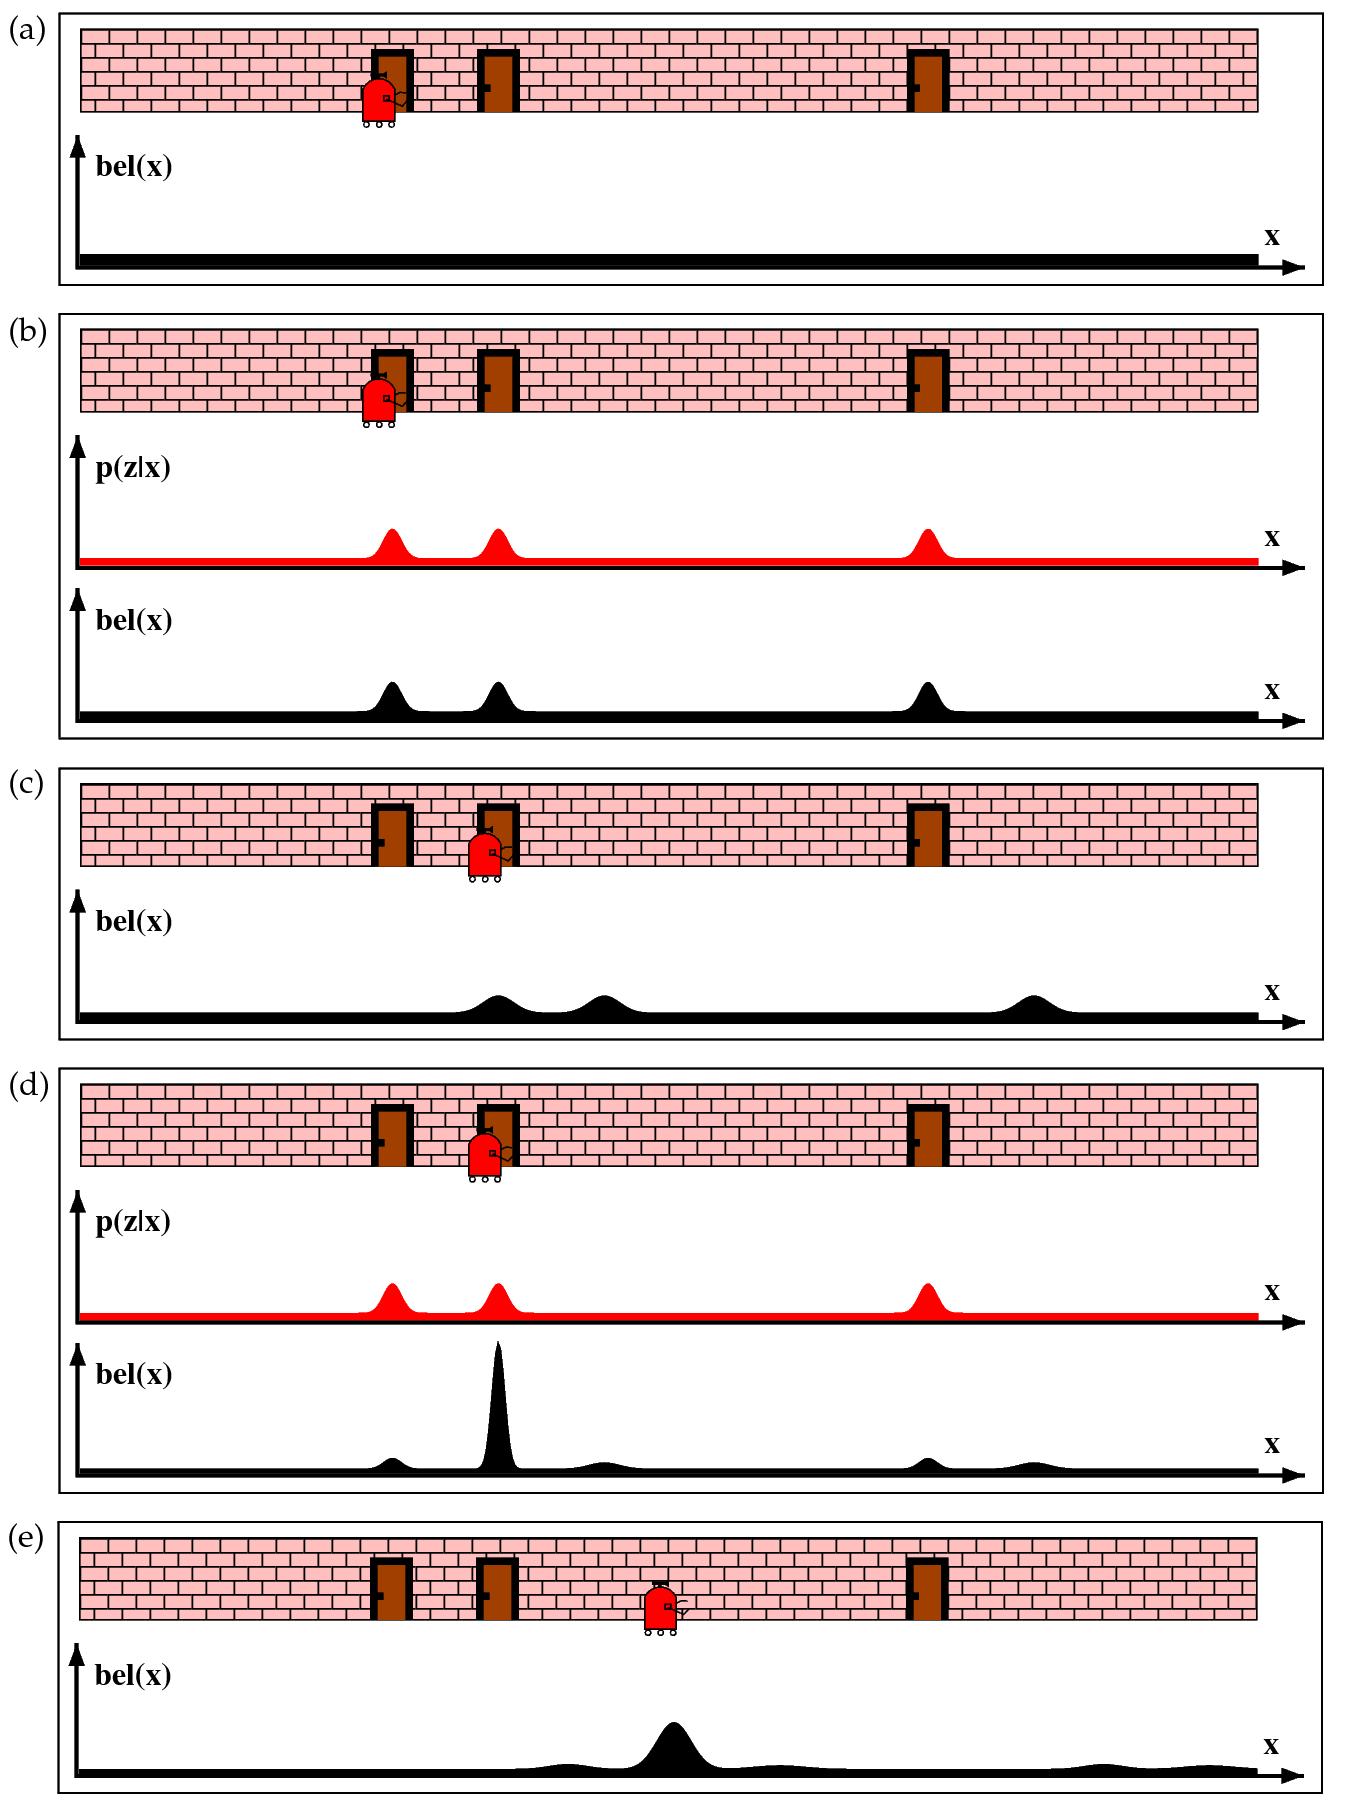
\includegraphics[width=.9\columnwidth]{pics/markov_localization}
  \caption{Markov localization. From \cite[p.~6]{ThrunBurgardFox:2005}.}
  \label{fig:markov_localization_one_dimension}
\end{figure}

A popular example for demonstrating Bayes' filters is the door example, which can be seen in figure \ref{fig:markov_localization_one_dimension}. A robot which can only move in one dimension and only sense whether it is in front of a door or not shall localize itself in a corridor. 

At the time of initialization the robot has no information, thus its believe to be at a specific position is uniformly distributed (see fig. \ref{fig:markov_localization_one_dimension}(a), $bel(x)$).

After the initialization the robot uses its sensor to search for a door. It finds out that in fact it is located in front of one, so it applies a high likelihood for all positions which are in front of doors (see fig. \ref{fig:markov_localization_one_dimension}(b), \p{x}{z} where $z$ denotes the sensor data). Now the prior belief $bel(x)$ and the likelihood \p{z}{x} are used to calculate the posterior belief \p{x}{z}, which is again called $bel(x)$.

\begin{align}
\p{x}{z} &= \eta\: \p{z}{x} bel(x) \label{eq:door_bayes}
\end{align}

A repeated measurement would add little information to the robot's belief. So the best solution to get more information is to move around a little and check for doors again. This can be seen in figure \ref{fig:markov_localization_one_dimension}(c). Especially noteworthy is that the $bel(x)$ distribution is flattened a little bit. This is done to account for inaccuracies in the movement of robots.

During the next time step the formula \ref{eq:door_bayes} will be used again, with the new---hence updated---belief and of course a new measurement. Since the robot again senses a door first it assigns high likelihoods for the doors, then it calculates the posterior belief. This leads to a considerable high value for the position close to the second door, we say the pose estimation converges to the real value. 

After the next movement the $bel(x)$ distribution flattens a little bit again, however it should get higher probabilities again when the robot senses no door at all.

\todo{some closing statement for the example, why this is a continuous example but we need a discrete version, what the differences are}

\section{}

\end{document}